\section{Auswertung}
\label{sec:Auswertung}

% % Examples
% \begin{equation}
%   U(t) = a \sin(b t + c) + d
% \end{equation}
%
% \begin{align}
%   a &= \input{build/a.tex} \\
%   b &= \input{build/b.tex} \\
%   c &= \input{build/c.tex} \\
%   d &= \input{build/d.tex} .
% \end{align}
% Die Messdaten und das Ergebnis des Fits sind in Abbildung~\ref{fig:plot} geplottet.
%
% %Tabelle mit Messdaten
% \begin{table}
%   \centering
%   \caption{Messdaten.}
%   \label{tab:data}
%   \sisetup{parse-numbers=false}
%   \begin{tabular}{
% % format 1.3 bedeutet eine Stelle vorm Komma, 3 danach
%     S[table-format=1.3]
%     S[table-format=-1.2]
%     @{${}\pm{}$}
%     S[table-format=1.2]
%     @{\hspace*{3em}\hspace*{\tabcolsep}}
%     S[table-format=1.3]
%     S[table-format=-1.2]
%     @{${}\pm{}$}
%     S[table-format=1.2]
%   }
%     \toprule
%     {$t \:/\: \si{\milli\second}$} & \multicolumn{2}{c}{$U \:/\: \si{\kilo\volt}$\hspace*{3em}} &
%     {$t \:/\: \si{\milli\second}$} & \multicolumn{2}{c}{$U \:/\: \si{\kilo\volt}$} \\
%     \midrule
%     \input{build/table.tex}
%     \bottomrule
%   \end{tabular}
% \end{table}
%
% % Standard Plot
% \begin{figure}
%   \centering
%   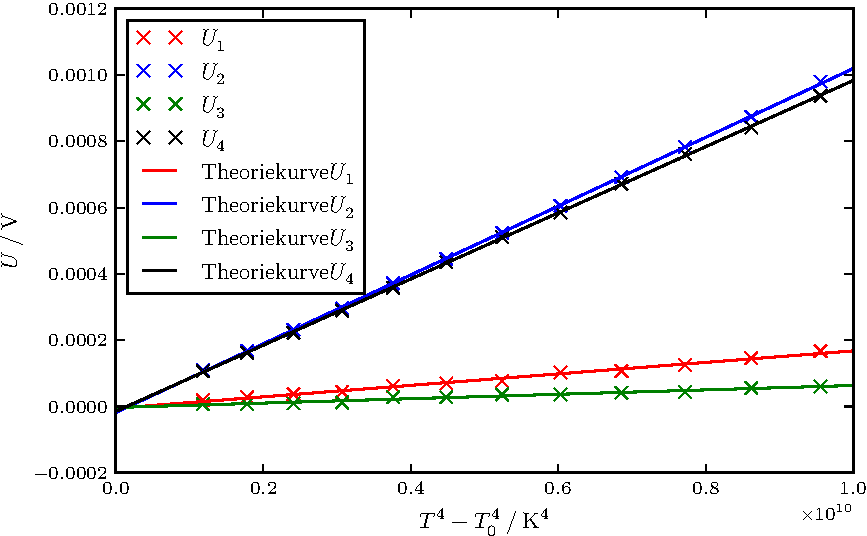
\includegraphics{build/plot.pdf}
%   \caption{Messdaten und Fitergebnis.}
%   \label{fig:plot}
% \end{figure}
%
% 2x2 Plot
% \begin{figure*}
%     \centering
%     \begin{subfigure}[b]{0.475\textwidth}
%         \centering
%         \includegraphics[width=\textwidth]{Abbildungen/Schaltung1.pdf}
%         \caption[]%
%         {{\small Schaltung 1.}}
%         \label{fig:Schaltung1}
%     \end{subfigure}
%     \hfill
%     \begin{subfigure}[b]{0.475\textwidth}
%         \centering
%         \includegraphics[width=\textwidth]{Abbildungen/Schaltung2.pdf}
%         \caption[]%
%         {{\small Schaltung 2.}}
%         \label{fig:Schaltung2}
%     \end{subfigure}
%     \vskip\baselineskip
%     \begin{subfigure}[b]{0.475\textwidth}
%         \centering
%         \includegraphics[width=\textwidth]{Abbildungen/Schaltung4.pdf}    % Zahlen vertauscht ... -.-
%         \caption[]%
%         {{\small Schaltung 3.}}
%         \label{fig:Schaltung3}
%     \end{subfigure}
%     \quad
%     \begin{subfigure}[b]{0.475\textwidth}
%         \centering
%         \includegraphics[width=\textwidth]{Abbildungen/Schaltung3.pdf}
%         \caption[]%
%         {{\small Schaltung 4.}}
%         \label{fig:Schaltung4}
%     \end{subfigure}
%     \caption[]
%     {Ersatzschaltbilder der verschiedenen Teilaufgaben.}
%     \label{fig:Schaltungen}
% \end{figure*}
\subsection{Bestimmung der Schallgeschwindigkeit in Acryl mittels Impuls-Echo-Verfahren}
Die Messung der einzelnen Zylinder mittels Schiebelehre ergibt die Zylinderhöhen
\begin{align*}
  h_1 &= \SI{61.5}{\milli\metre}, \\
  h_2 &= \SI{80.55}{\milli\metre}, \\
  h_3 &= \SI{102.1}{\milli\metre}, \\
  h_4 &= \SI{120.5}{\milli\metre}, \\
  h_5 &= \SI{31.3}{\milli\metre}.
\end{align*}
Die Durchführung eines Impuls-Echo-Verfahren ergibt die in Tabelle \ref{tab:0} dargestellten Laufzeiten $\increment t$ zu den jeweiligen Zylinderhöhen $h$.
Hierbei werden zunächst alle Zylinder einzeln und zum Schluss zwei Kombinationen aus $h_5$ und $h_1$ bzw. $h_2$ betrachtet.
Aus dem Weg-Zeit-Gesetz wird somit die jeweilige Geschwindigkeit des Impulses berechnet, wobei aufgrund der Reflektion die doppelte Weglänge berücksichtigt werden muss.
  \begin{table}
    \centering
    \caption{Bestimmung der Schallgeschwindigkeit mittels Impuls-Echo-Verfahren.}
    \label{tab:0}
    \sisetup{parse-numbers=false}
    \begin{tabular}{
	S[table-format=3.2]
	S[table-format=2.1]
	S[table-format=4.2]
	}
	\toprule
	{$h_{\text{zylinder}} \:/\: 10^{-3} \si{\metre}$}		& {$\increment t \:/\: 10^{-6} \si{\second} $}		& 
	{$c_\text{Acryl} \:/\: \si{\metre\per\second} $}		\\ 
	\midrule
    61.50  & 44.9 & 2739.42 \\
80.55  & 58.3 & 2763.29 \\
102.10 & 75.0 & 2722.67 \\
120.50 & 87.4 & 2757.44 \\
92.60  & 67.8 & 2731.56 \\
111.85 & 81.1 & 2758.32 \\

    \bottomrule
    \end{tabular}
    \end{table}

Die Bestimmung der Mittelwertes nach Formel \eqref{eq:std_mean} sowie die Bestimmung des Fehler nach Formel \eqref{eq:std} ergibt somit eine gemittelte Schallgeschwindigkeit in Acryl von
\begin{align*}
  c_{\text{acryl,e}} &= \SI{2745+-15}{\metre\per\second}
.\\
\end{align*}

Die genauere Betrachtung der ersten Messung ergibt eine Amplitude des ersten Peaks von
\begin{align*}
  U_1 = \SI{1.214}{\volt}

\end{align*}
sowie eine Amplitude des zweiten Peaks von
\begin{align*}
  U_2 = \SI{1.105}{\volt}
.
\end{align*}
Die Peaks werden zu den Laufzeiten
\begin{align*}
  t_1 = \SI{1.3}{\micro\second}

\end{align*}
beziehungsweise
\begin{align*}
  t_2 = \SI{46.2}{\micro\second}

\end{align*}
gemessen.
Hieraus ergibt sich die zuvor in Tabelle \ref{tab:0} angegebene Laufzeitdifferenz.
Bei Eingabe der berechneten Schallgeschwindigkeit in das Auswertungsprogramm ergibt sich für die Tiefenmessung exakt die mit der Schiebelehre gemessene Länge des Zylinders, was die Funktion des Programmes bestätigt. %duh

\subsubsection{Ausgleichsrechnung zur Bestimmung des systematischen Fehlers}
Aufgrund der endlichen Dicke der Anpassungsschicht der Sonde tritt ein systematischer Fehler auf.
Um diesen zu ermitteln, werden die gemessenen Weglängen gegen die halbierten Laufzeiten aufgetragen und ein linerer Fit durchgeführt.
Der Grund der halbierten Laufzeiten ist wiederum die effektive doppelte Weglänge, die zurückgelegt werden muss.
Diese wird in Python mit Numpy mittels der Methode der kleinsten Quadrate durchgeführt.
Es ergibt sich der in Abbildung \ref{fig:plot1} dargstellte Graph.
\begin{figure}
  \centering
  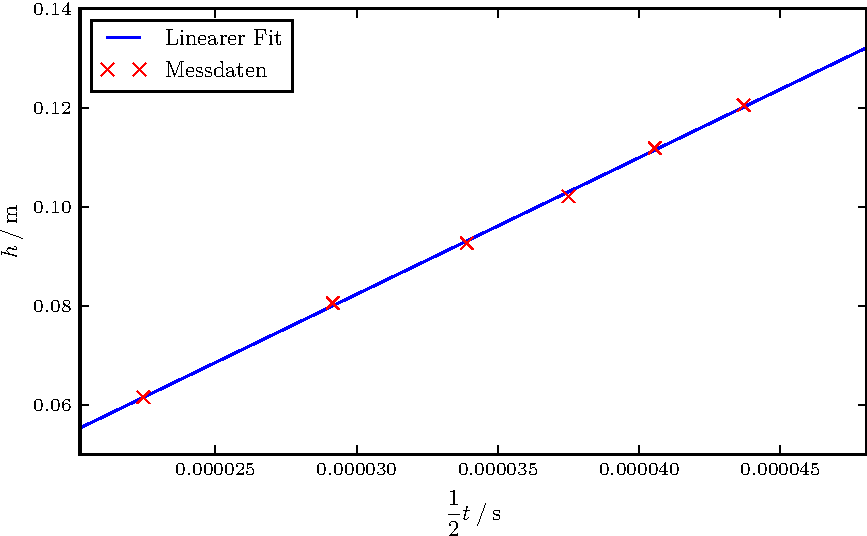
\includegraphics{build/ausgleich.pdf}
  \caption{Ausgleichsrechnung zur Bestimmung der Dicke der Anpassungsschicht.}
  \label{fig:plot1}
\end{figure}
Die ermittelten Fitparameter sind dabei
\begin{align*}
  m &= \SI{2760+-38}{\metre\per\second}
 \\
  b &= \SI{-0.0005+-0.0013}{\metre}
.
\end{align*}
Die Steigung lässt sich hierbei identifizieren als Wert für die Schallgeschwindigkeit in Acryl, der Achsenabschnitt beschreibt den systematischen Fehler, bzw. die Dicke der Anpassungsschicht.

\subsection{Bestimmung der Schallgeschwindigkeit in Acryl mittels Durchschallungs-Methode}
Für die Messungen mit der Durchschallungs-Methode ergeben sich die Werte aus Tabelle \ref{tab:1}, wobei die Computer-Software die Messung für größere Zylinder nicht möglich gemacht hat.
  \begin{table}
    \centering
    \caption{Bestimmung der Schallgeschwindigkeit mittels Durchschallungs-Methode.}
    \label{tab:1}
    \sisetup{parse-numbers=false}
    \begin{tabular}{
	S[table-format=2.2]
	S[table-format=2.1]
	S[table-format=4.2]
	}
	\toprule
	{$h_{\text{zylinder}} \:/\: 10^{-3} \si{\metre}$}		& {$\increment t \:/\: 10^{-6} \si{\second} $}		& 
	{$c_\text{Acryl} \:/\: \si{\metre\per\second} $}		\\ 
	\midrule
    31.30 & 11.5 & 2709.96 \\
61.50 & 22.8 & 2697.37 \\
80.55 & 30.4 & 2645.32 \\

    \bottomrule
    \end{tabular}
    \end{table}

Mit Hilfe dieser wird die gemittelte Schallgeschwindigkeit in Acryl auf
\begin{align*}
  c_{\text{acryl,d}} &= \SI{2684+-28}{\metre\per\second}
\\
\end{align*}
bestimmt.

\subsection{Bestimmung des Abschwächungskoeffizienten von Acryl}
Aus den Werten der Intensitätspeaks und Laufzeiten der Echo-Impuls Messung kann der Schwächungskoeffizient $\alpha$ nach Gleichung \ref{gl:1} auf die Weise
\begin{equation}
  \alpha = \frac{\ln{\frac{U_1}{U_2}}}{t_1-t_2}
\end{equation}
berechnet werden.
Somit ergibt sich
\begin{align*}
  \alpha &= \SI{-2095.2}{\second\tothe{-1}}
.\\
\end{align*}
